% ch04-literature.tex – Chapter 4: literature review and the flagship paper.
% Round 1 (Writer): flagship-paper sections only. Thematic review (§4.1) follows in round 2.
\ChapterMission{המשימה: להבין מה בדיוק מדד מאמר הדגל, מה אפשר להסיק ממנו ומה עדיין חסר}
\ChapterIcon{sensor}
\chapter{סקירת ספרות ומאמר הדגל}
\begin{scenebox}
אותו מעבר חציה, שעת העומס של הבוקר. על המדרכה מצטופפים שבעה או שמונה אנשים, וכולם מביטים באיש האדום.
גבר אחד מתקדם חצי צעד אל הכביש, מסתכל סביבו ונסוג בחזרה אל השפה.
איש לא אמר לו מילה. האור עדיין אדום.
\end{scenebox}

השאלה שהתמונה הזו מעלה, האם עצם נוכחותם של אחרים על המדרכה מרסנת את ההחלטה לחצות באדום, היא שאלת המחקר של מאמר הדגל.
הפרק מציג את המאמר ואת ממצאיו, בוחן באופן ביקורתי את הנתונים שפורסמו בו ומגדיר את פער הידע שהפרויקט נועד לגשר עליו.

\section{סקירה תמטית}
% TODO round 2: thematic review (Researcher sources)

\section{מאמר הדגל: חצייה באדום, יחידים וקבוצות}
המחקר של רוזנבלום \cite{rosenbloom2009} נבחר כמאמר הדגל משלוש סיבות.
הוא נערך בצומת עירוני בתל אביב, כלומר בהקשר שבו אמורה לפעול המערכת המוצעת;
הוא בודק לא רק מי חוצה באדום אלא כיצד מספר הממתינים על המדרכה משפיע על ההחלטה, וזו בדיוק הנקודה שבה מערכת חישה יכולה להתערב;
והוא מפרסם את נתוני הספירה ואת מקדמי המודל, כך שאפשר לבדוק אותם מחדש.
המאמר נשען על תאוריית השליטה החברתית (\en{social control}), שלפיה אדם הממתין לבדו חש מחויבות חלשה יותר לנורמה מאשר אדם המוקף באחרים.

\paragraph{שיטה.}
זהו מחקר תצפית שדה, שבו ההולכים לא ידעו שהם נצפים \cite{rosenbloom2009}.
שני צופים מיומנים עמדו בצד הדרך ותיעדו כל הולך רגל שהגיע אל מעבר חציה מרומזר אחד, בשמונה מפגשים בני שעה בין \num{07:30} ל-\num{08:30}.
בטופס תצפית מובנה (\en{observation grid}) נרשמו לכל הולך מגדר, קבוצת גיל משוערת, צבע הרמזור בהגעה ובחצייה, מספר הממתינים שכבר עמדו על המדרכה, מספר המצטרפים אחריו, נפח התנועה והאם אדם אחר חצה באדום באותו מופע.
המשתנה התלוי היה דו-ערכי: חצה באדום או המתין לירוק.
בסך הכול נצפו \num{1,392} הולכי רגל, מהם \num{842} נשים (\pct{60.5}) ו-\num{550} גברים (\pct{39.5}).

\paragraph{ממצאים.}
\num{563} מן הנצפים (\pct{40.4}) הגיעו כשהרמזור אדום, ו-\num{76} מהם חצו באדום: \pct{5.5} מכלל התצפיות, אך \pct{13.5} ממי שהגיעו באדום, ורק להם ההחלטה הייתה אפשרית.
איור~\ref{fig:g1} מראה שבקבוצה זו שיעור החוצים בקרב גברים, \pct{20.6} (\num{48} מתוך \num{233}), גבוה פי שניים ויותר מאשר בקרב נשים, \pct{8.5} (\num{28} מתוך \num{330}).
ההבדל מובהק, \num{$\chi^2(1, N=563) = 17.17$}, והערך משתחזר במדויק מנתוני הספירה שבמאמר \cite{rosenbloom2009}.

\begin{figure}[ht]
  \centering
  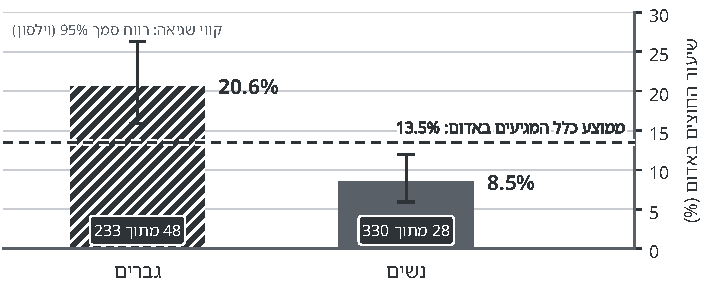
\includegraphics[width=\linewidth]{figures/g1-crossing-by-gender.pdf}
  \caption{שיעור החוצים באדום בקרב מי שהגיעו במופע האדום, לפי מגדר (עובד מתוך \cite{rosenbloom2009})}
  \label{fig:g1}
\end{figure}

כדי לבחון כמה גורמים יחד, המחבר התאים לקבוצת המגיעים באדום מודל רגרסיה לוגיסטית (\en{logistic regression}), המתאר את הלוגריתם של יחס הסיכויים לחצייה באדום כצירוף ליניארי של המנבאים (משוואה~\eqref{eq:logit}):
\begin{equation}
  \ln\frac{p}{1-p} = \beta_0 + \beta_1 x_{\hebmath{מגדר}} + \beta_2 x_{\hebmath{ממתינים}} + \beta_3 x_{\hebmath{מצטרפים}} + \beta_4 x_{\hebmath{תנועה}} + \beta_5 x_{\hebmath{חוצה אחר}}
  \label{eq:logit}
\end{equation}
כאן $p$ היא ההסתברות שהולך שהגיע באדום יחצה באדום. מקדם מתורגם ליחס סיכויים (\en{odds ratio}) לפי $\mathrm{OR}_i = e^{\beta_i}$: ערך מעל \num{1} מגדיל את הסיכויים, וערך מתחתיו מקטין אותם.
לפי המודל, הסיכויים של גבר לחצות באדום גבוהים פי \num{3.71} משל אישה, וכל אדם נוסף הממתין על המדרכה או מצטרף אליה מקטין אותם.
נפח התנועה וחצייה של אדם אחר באדום לא נמצאו מנבאים מובהקים \cite{rosenbloom2009}.
מכאן מסקנת המאמר: הקבוצה הממתינה מפעילה שליטה חברתית, וככל שעל המדרכה יותר אנשים, כך פחות אנשים חוצים באדום.

\begin{statrow}[3]
  \stattile[SignalRed]{\pct{13.5}}{מהמגיעים במופע האדום חצו באדום}
  \stattile[SignalAmber]{\num{3.71}}{יחס הסיכויים לחצייה באדום של גבר לעומת אישה}
  \stattile[SignalGreen]{\num{0.63}}{יחס הסיכויים לכל ממתין נוסף (מחושב מחדש)}
\end{statrow}

\section{ניתוח ביקורתי של הנתונים}
כל הערכים בטבלאות המאמר הוקלדו מחדש, נבדקו מול העמוד המודפס וחושבו מחדש בסקריפט.
הבדיקה העלתה שש סוגיות, המסוכמות בתיבה שלהלן. הן אינן מבטלות את כיוון הממצא המרכזי, אך משנות את גודל האפקט ואת מה שמותר להסיק ממנו.

\begin{cautionbox}
\begin{itemize}
\item \en{D1}: עמודת \en{$e^{b}$} אינה תואמת את \en{$\exp(b)$} בשני מנבאים: ממתינים (\num{0.71} במקום \num{0.63}) ומצטרפים (\num{0.67} במקום \num{0.63}).
\item \en{D2}: שורת נפח התנועה סותרת את עצמה: המקדם ושגיאת התקן מצביעים על אפקט זניח, ואילו יחס הסיכויים, רווח הסמך ומבחן \en{Wald} מצביעים על אפקט מובהק.
\item \en{D3}: פרק התוצאות קובע ששתי ההשערות נדחו, ואילו פרק הדיון קובע שההשערה הראשונה אוששה.
\item \en{D4}: מקדם החצייה של הולך רגל אחר אינו ניתן לפירוש (הפרדה מלאה במודל).
\item \en{D5}: שני אחוזים מודפסים אינם תואמים את הספירות.
\item \en{D6}: מגבלות שיטה: אתר אחד, שעה אחת, תצפיות תלויות וללא מדידת זמן המתנה.
\end{itemize}
\end{cautionbox}

איור~\ref{fig:g2} משווה לכל מנבא את יחס הסיכויים ורווח הסמך שפורסמו לערכים המחושבים מן המקדם $b$ ומשגיאת התקן.
במגדר הערכים זהים. בממתינים ובמצטרפים רווחי הסמך תואמים את המקדמים, אך יחס הסיכויים אינו תואם (\en{D1}):
כל ממתין נוסף מקטין את הסיכויים לחצייה באדום בכ-\pct{37}, ולא בכ-\pct{29}. הכיוון נשמר, והאפקט אף חזק מעט יותר.
בשורת נפח התנועה (\en{D2}) מן $b = -0.03$ ושגיאת תקן \num{0.03} מתקבל יחס סיכויים \num{0.97} ורווח סמך \range{0.92}{1.03}, כלומר אפקט לא מובהק;
ואילו יחס הסיכויים שפורסם (\num{2.20}), רווח הסמך שלו ומבחן \en{Wald} (\num{6.06}) עקביים זה עם זה, אך מחייבים $b \approx 0.79$ ואפקט מובהק, בניגוד לטקסט התוצאות.
מתוך המאמר אי אפשר להכריע איזו גרסה נכונה, ולכן הדוח אינו נשען על שורה זו.

\begin{figure}[ht]
  \centering
  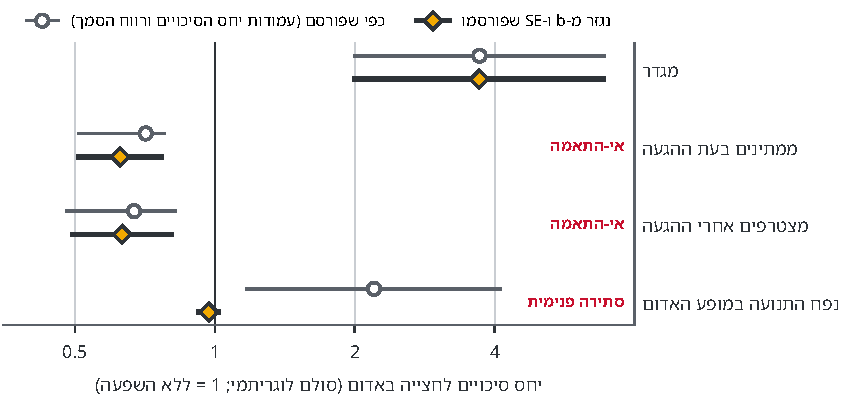
\includegraphics[width=\linewidth]{figures/g2-odds-ratios.pdf}
  \caption{יחסי הסיכויים ורווחי הסמך: כפי שפורסמו לעומת חישוב מחדש מן המקדמים (עובד מתוך \cite{rosenbloom2009})}
  \label{fig:g2}
\end{figure}

בסוגיה \en{D3}, המקדמים השליליים של הממתינים והמצטרפים תומכים בהשערה הראשונה, שלפיה יחידים חוצים באדום יותר מאנשים בקבוצה, ולכן נראה שהמשפט בפרק התוצאות הוא הטעות.
גם הדיון בהשערה השנייה אינו עקבי: נטען בו שחצייה של אדם אחד עשויה לעודד אחרים, ומיד לאחר מכן מדווח שהנצפים לא הושפעו ממנה \cite{rosenbloom2009}.
סוגיה \en{D4} מסבירה מדוע השערה זו אינה ניתנת לבדיקה: מקדם של \num{$-$24.24} עם שגיאת תקן של \num{8,184.53} הוא סימן להפרדה מלאה או כמעט מלאה (\en{quasi-complete separation}), מצב שבו המודל אינו מסוגל לאמוד את המקדם.
בסוגיה \en{D5}, שיעור הנשים בקרב החוצים בירוק מודפס כ-\pct{60.8}, ואילו מן הספירה (\num{512} מתוך \num{829}) מתקבל \pct{61.8}, ושיעור בני \range{20}{40} מופיע כ-\pct{94.4} בטבלה וכ-\pct{94.3} בפרק השיטה; כל שאר הערכים המרכזיים משתחזרים במדויק.

סוגיה \en{D6} עוסקת בתוקף: מעבר אחד, שעת בוקר אחת, גיל שהוערך במבט, ואי-יכולת להבחין בין קבוצה שהגיעה יחד לבין זרים שהמתינו זה לצד זה \cite{rosenbloom2009}.
הולכים הממתינים באותו מופע גם אינם תצפיות בלתי תלויות, בעוד המודל הלוגיסטי מניח אי-תלות, ולכן ייתכן שרווחי הסמך צרים מן הראוי.
בנוסף, המאמר אינו מדווח על החותך $\beta_0$ שבמשוואה~\eqref{eq:logit}, ובלעדיו אי אפשר לחשב את ההסתברות המוחלטת $p$ לחצייה באדום, אלא רק יחסים בין מצבים.
לכן איור~\ref{fig:g3} מציג סיכויים יחסיים בלבד: הסיכויים של מי שמגיע אל מדרכה שעליה ממתינים $k$ אנשים, ביחס למגיע אל מדרכה ריקה, לפי $\mathrm{OR}^{k}$.
העקומה מראה כיצד האפקט מצטבר, כך שכבר עם שלושה ממתינים הסיכויים יורדים לכרבע בערך, אך אינה מראה מה שיעור החוצים בפועל.

\begin{figure}[ht]
  \centering
  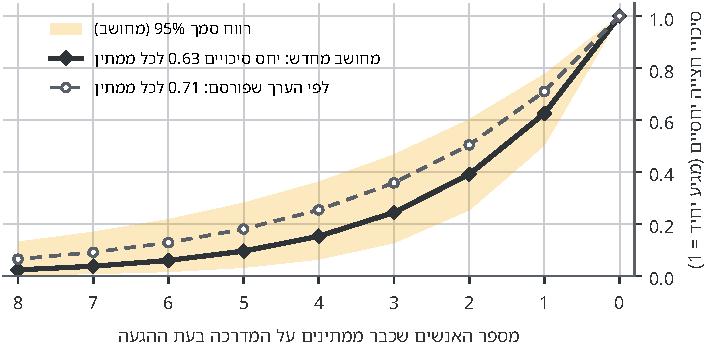
\includegraphics[width=\linewidth]{figures/g3-relative-odds.pdf}
  \caption{סיכויי חצייה יחסיים לפי מספר הממתינים בעת ההגעה, ביחס למגיע יחיד (עובד מתוך \cite{rosenbloom2009})}
  \label{fig:g3}
\end{figure}

\section{פער הידע}
המאמר מבסס את הטענה שהקבוצה על המדרכה מרסנת חצייה באדום, אך משאיר שלושה פערים שהם נקודת המוצא של הפרויקט.
הראשון הוא זמן ההמתנה: איש לא מדד כמה שניות עברו מן ההגעה ועד ההחלטה, והמחבר עצמו מציע לעשות זאת בתוכנת תזמון או בצילום וידאו \cite{rosenbloom2009}.
השני הוא היקף התצפית: אתר אחד ושעה אחת אינם מלמדים על שעות, צמתים ואוכלוסיות אחרים.
השלישי הוא המעבר מתיאור להתערבות: המאמר ממליץ על רמזורים המציגים את הזמן שנותר, אך אינו בוחן אמצעי טכנולוגי כלשהו.
חיישן הסופר ממתינים ומודד זמני המתנה, יחד עם תצוגת ספירה לאחור (\en{countdown}), יכול גם לאסוף את הנתונים החסרים וגם לבחון את ההמלצה בשטח.

\begin{findingbox}
מאמר הדגל מראה שכל אדם נוסף הממתין על המדרכה מקטין את הסיכויים לחצייה באדום, אך אינו מודד זמני המתנה, נשען על אתר אחד ואינו מאפשר לחשב הסתברות מוחלטת.
מערכת המשלבת חישת ממתינים, מדידת זמן המתנה ותצוגת ספירה לאחור עונה ישירות על שלושת הפערים האלה.
\end{findingbox}
